%!TEX root = ../thesis.tex

\chapter{Results}
\label{chap:r}

\textit{[Chapter intro to be written.]}

\subsection{Manual pre-processing}
\label{sub:manualpreprocessing}

Implementing a scaling solution did not form part of this project, although all parts of the implementation were designed in a way that a binary production version of it would have manageable computational complexity and could be embedded in a scaling framework with a relatively small amount of effort. Scaling in this project concerns primarily the need to subdivide the input data in a way that the software can queue up portions of it for parallel computation and never run out of memory while processing a set number of these portions. These portions could be generated, in the simplest case, based on tiling, i.e. overlaying a 2D raster on the extents of the data and examining which cell certain features fall into. 

As scaling was not part of this project, the task of creating such manageable subsets of the input data was carried out manually prior to starting development on the main processing steps. This procedure consisted of cropping the input vector datasets into tiles showing interesting 3D features (important for testing), and for each of them, retaining only those Lidar points which fall within their extents \textit{and} are a set maximum distance from any roads in their respective NWB tiles. For the former task, I used the vector operations toolset in QGIS, and for the latter I used LASTools. I derived the area of interest in which to keep Lidar points by buffering the centrelines in NWB tiles by 50 metres (?), and passing these geometries on to LASTools to crop AHN3 tiles. AHN3 itself comes tiled in the official release (on a much larger scale), and I derived each testing dataset from a single AHN3 tile to keep the manual procedure simple. I also discarded AHN3 points not classed as ground or bridge points, since these are the only points in AHN3 that could be relevant to the task of characterising road surfaces. This is explained in more depth in Section [REF]. Ultimately, the process resulted in 11 testing datasets, each with its own cropped NWB, DTB and AHN3 files.

\subsection{Testing datasets}
\label{sub:testingdata}

\textit{[Subsection to be written.]}

\textit{[Content below copied from P2; to be adapted.]}

Due to its volume, it will not be possible to develop and test the implementation without cropping AHN3 input point cloud tiles. Even after the implementation of the segmentation workflow, the size of the testing point clouds will need to be manageable, to facilitate efficient debugging. At the same time, they will need to be representative enough to provide an insight into the computational complexity and visual performance of the algorithm. I have already produced a range of testing datasets by selecting various lengths of NWB centrelines at interesting road features, and keeping only those Lidar points which are within a 150-metre buffer distance from the selected road centrelines. Table \ref{tab:inventory} provides an inventory of these. The tile identifier in the first column refers to those used in \cite{ahn3_download}. The resulting datasets fit into memory easily, even when extracted to LAS.

\begin{longtable}[c]{@{}p{2.8cm}p{6.8cm}c@{}}
\toprule
Title, tile  & Features & Render \\ \midrule
Markerwarddijk, 20BN1 & Dike-based P-road in the Markermeer. Very limited amount of terrain around the road. Road consistently build on ground, with no involvement of bridge structures. & \raisebox{-0.94\totalheight}{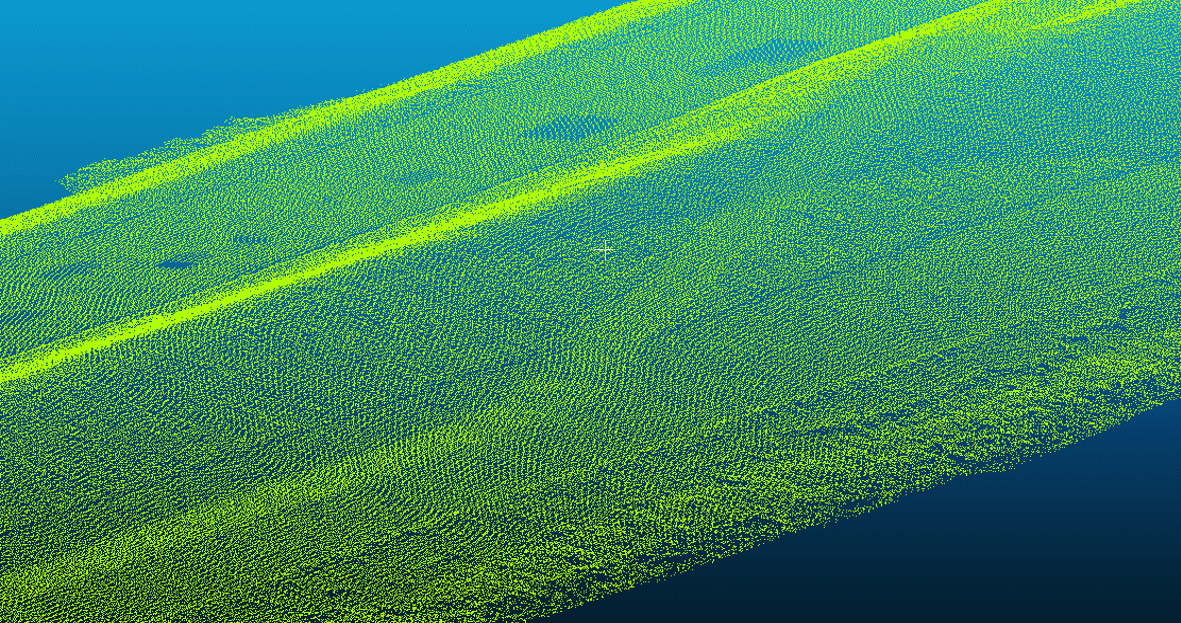
\includegraphics[width=6cm, height=3.5cm]{final_report/figs/ahn_sample_20BN1_a.png}}  \\
Amsterdam Hemhavens, 25BZ2 & Ringweg-West (R-road) as it crosses the IJ through the Coentunnel in a densely built-up environment. It is built on artificially elevated ground and on bridges in this area. Part of Westradweg also included, which has been built entirely on a long bridge. & \raisebox{-0.94\totalheight}{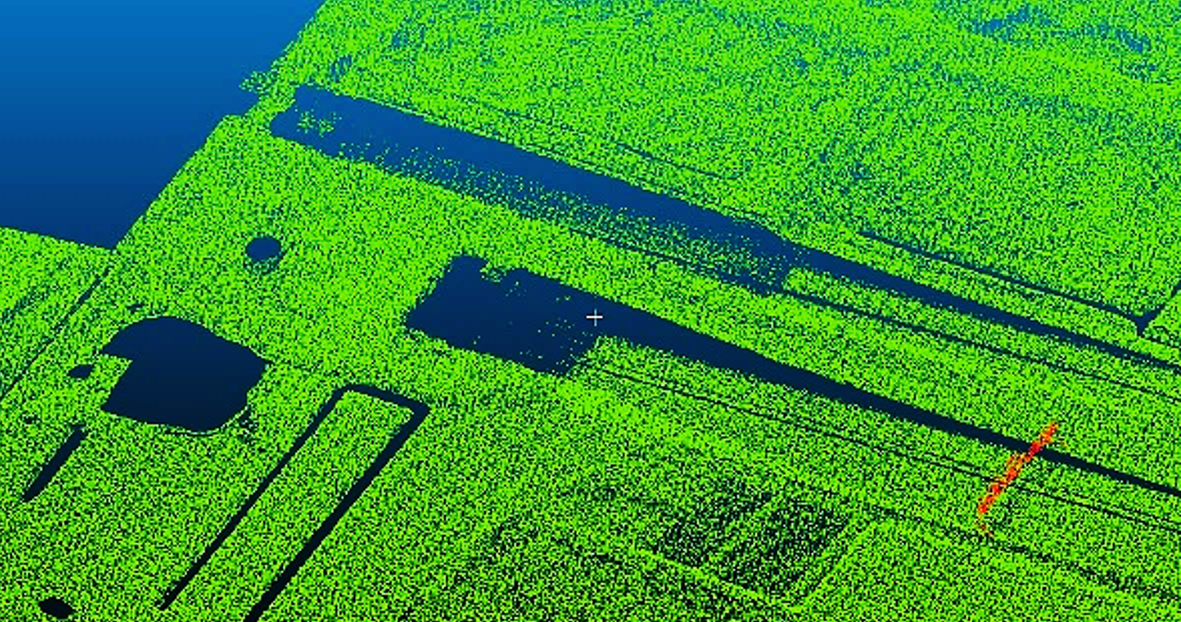
\includegraphics[width=6cm, height=3.5cm]{final_report/figs/ahn_sample_25BZ2_a.png}} \\
Amsterdam Zuid, 25DN2 & R-roads with many closely spaced bridges, small tunnels, dense grouping of holes around roads due to presence of water and buildings & \raisebox{-0.94\totalheight}{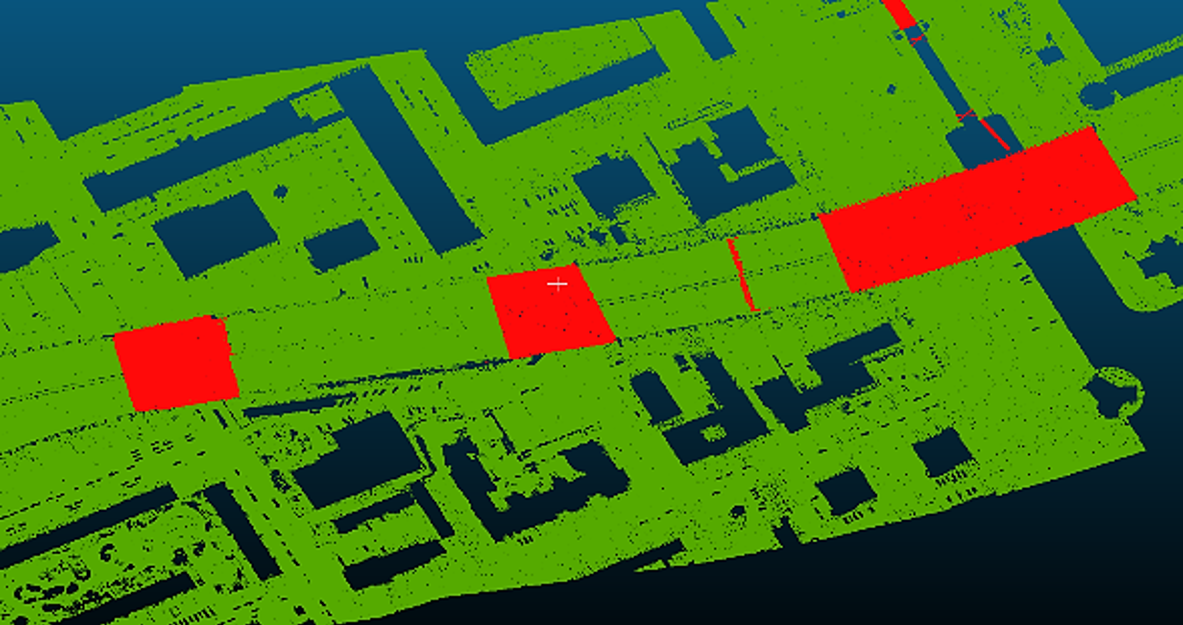
\includegraphics[width=6cm, height=3.5cm]{final_report/figs/ahn_sample_25DN2_a.png}} \\
Bunschoten, 32BN1 & P-roads with three big roundabouts, and one road that ends in a small roundabout. Amersfoortseweg has its two lanes on separate roads surfaces (like motorways), but with frequent connecting segments. & \raisebox{-0.94\totalheight}{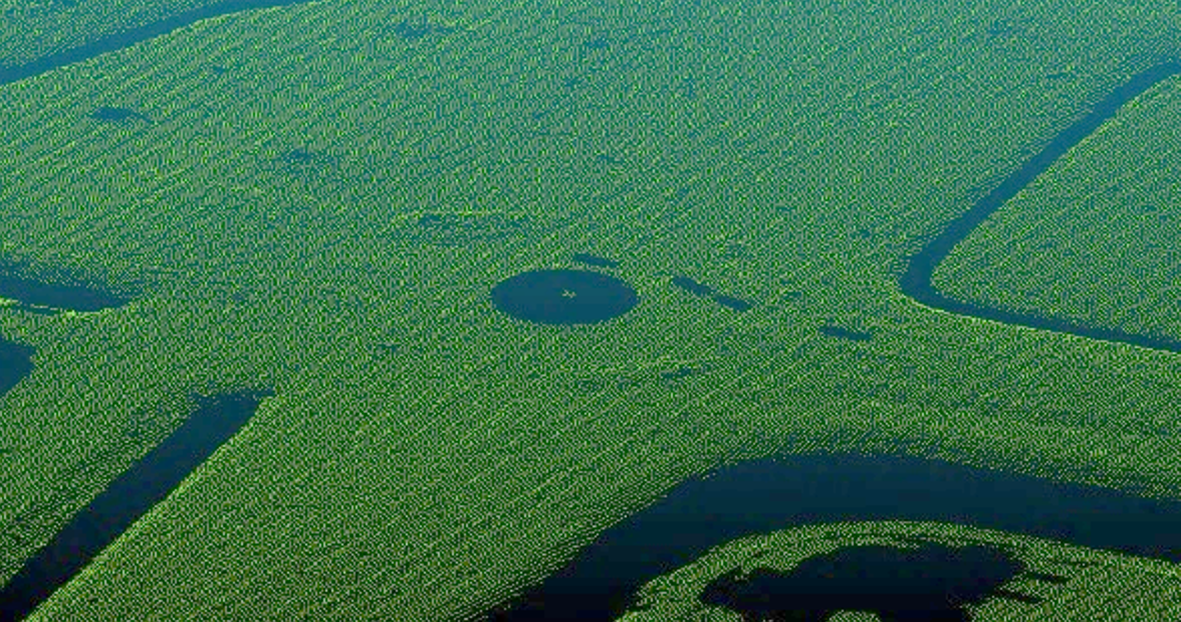
\includegraphics[width=6cm, height=3.5cm]{final_report/figs/ahn_sample_32BN1_a.png}} \\
Veluwe, 32FZ2 & Straight R-roads surrounded by dense forest and crossed by wide wildlife overpasses. & \raisebox{-0.94\totalheight}{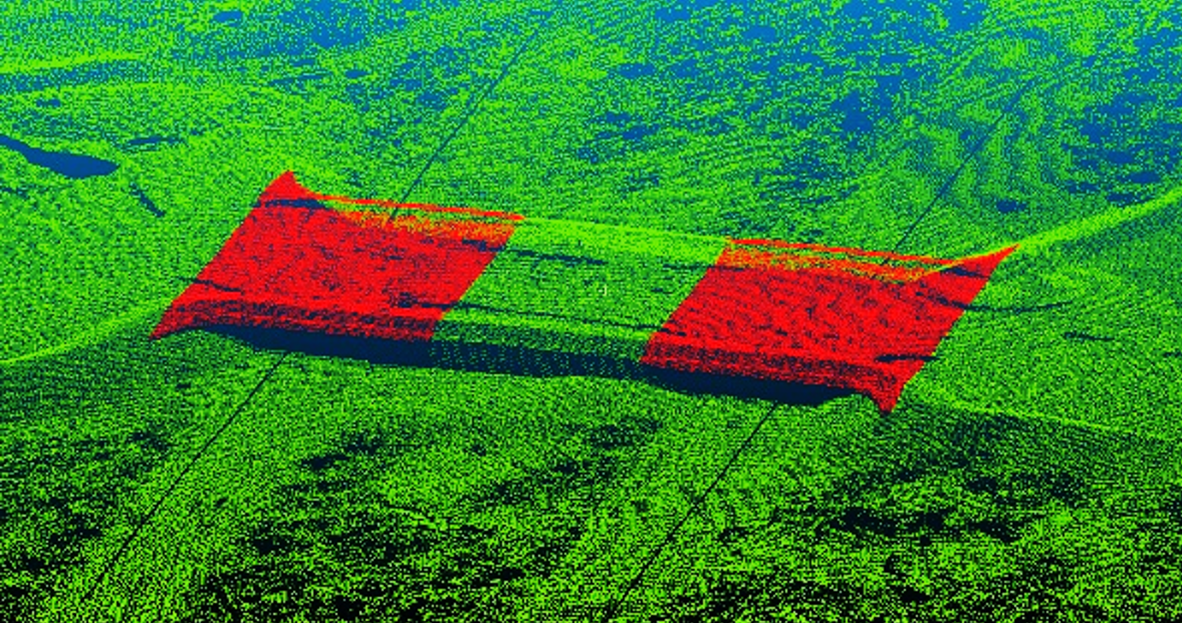
\includegraphics[width=6cm, height=3.5cm]{final_report/figs/ahn_sample_32FZ2_a.png}} \\
Apeldoornseweg, 32HZ2 & P-road in dense forest with canopy frequently occluding the road surface, decreasing point density and occasionally creating gaps. The road has small parallel branches running very close to it, which may make it difficult for the algorithm to distinguish between them. It also has roundabouts. & \raisebox{-0.94\totalheight}{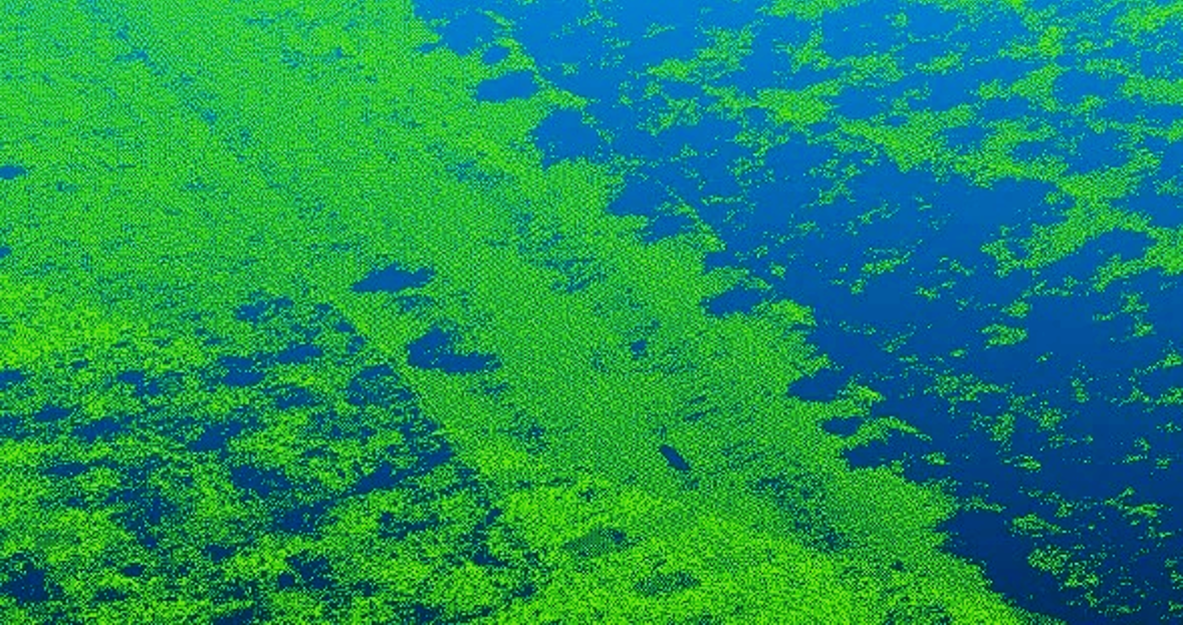
\includegraphics[width=6cm, height=3.5cm]{final_report/figs/ahn_sample_32HZ2_a.png}} \\
Hoenderloo, 33CN2 & P-road in extremely dense, continuous forest with canopy frequently occluding the road surface, decreasing point density and occasionally creating gaps. Both lanes are on the same road surface & \raisebox{-0.94\totalheight}{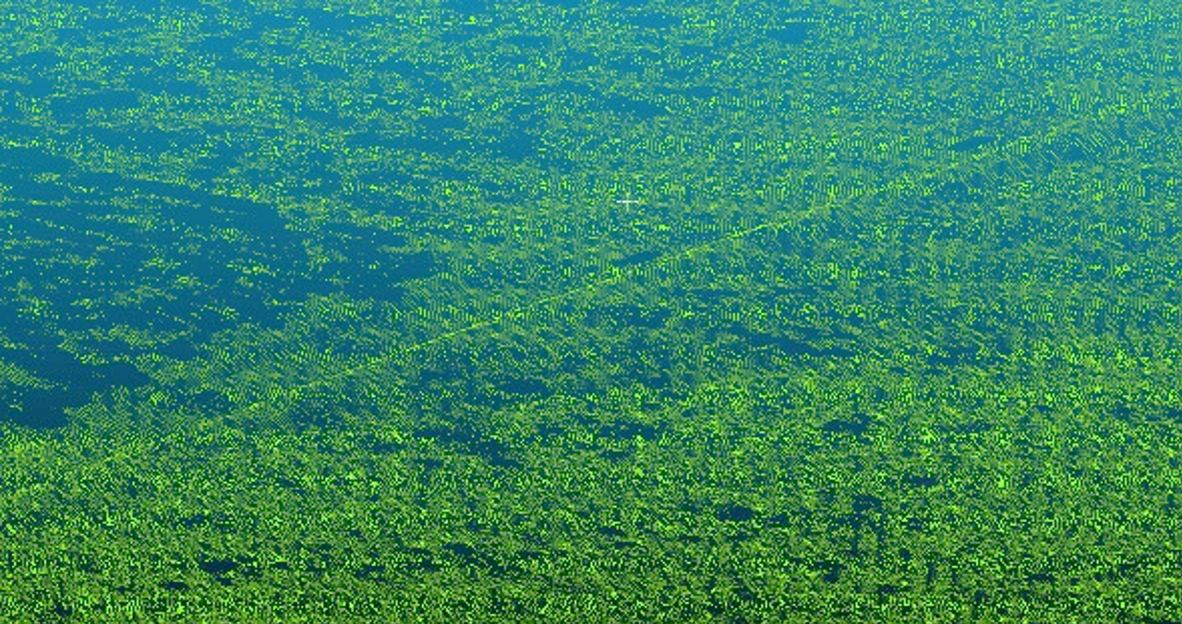
\includegraphics[width=6cm, height=3.5cm]{final_report/figs/ahn_sample_33CN2_a.png}} \\
Rotterdam Ketheltunnel, 37EZ1 & This segment of the A4 heading North from Rotterdam has been recently reconstructed in an underground tunnel. In addition, a significant portion of this R-road now runs in a trench towards Delft. AHN3 was imaged during the reconstruction, and hence contains erratic data about the road surface. & \raisebox{-0.94\totalheight}{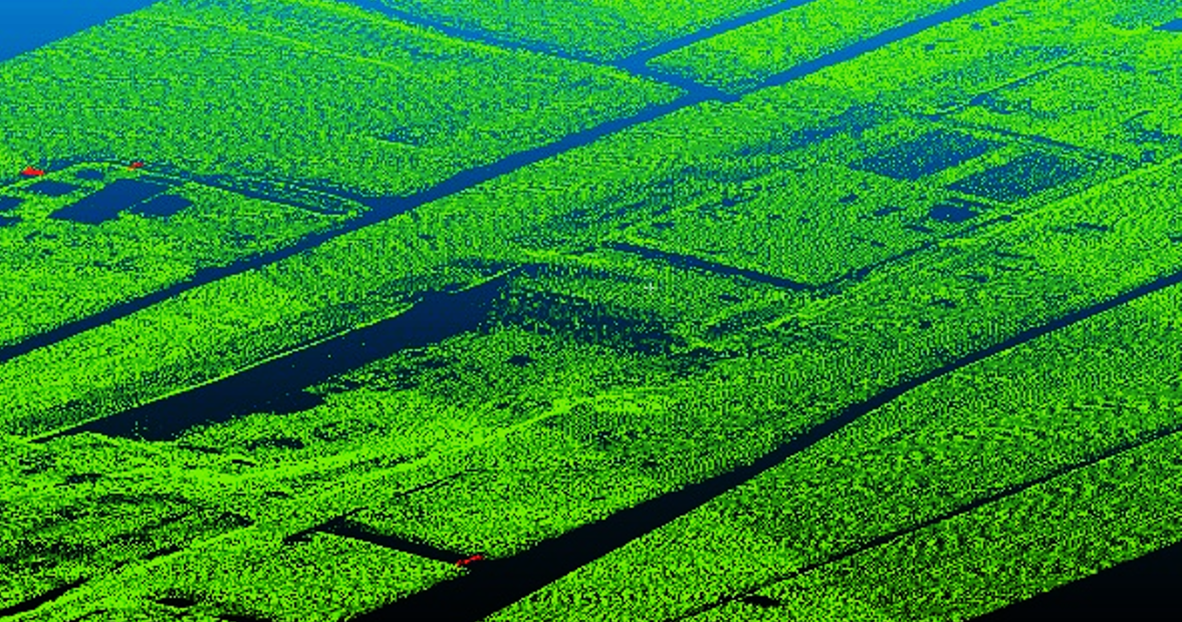
\includegraphics[width=6cm, height=3.5cm]{final_report/figs/ahn_sample_37EZ1_a.png}} \\
Knoppunt Ridderkerk, 37HN2 & The Ridderkerk interchange is one of the largest of its kind in The Netherlands, in one place containing 4 overlapping R-roads. Furthermore, it contains an extremely high density of R-roads in a small area, many of them very tightly packed in small areas. Many are intensely curved. & \raisebox{-0.94\totalheight}{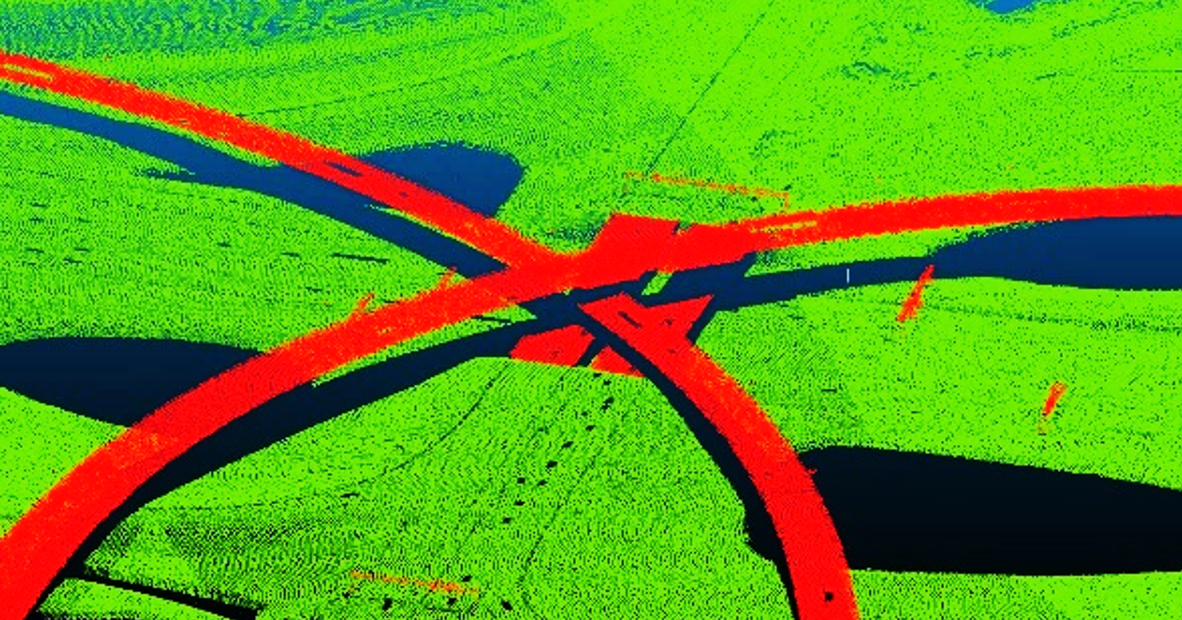
\includegraphics[width=6cm, height=3.5cm]{final_report/figs/ahn_sample_37HN2_a.png}} \\
Gorinchem, 38GZ1 & Complex interchange between a P-road and an R-road with small ramps, roundabouts and overlapping geometries. & \raisebox{-0.95\totalheight}{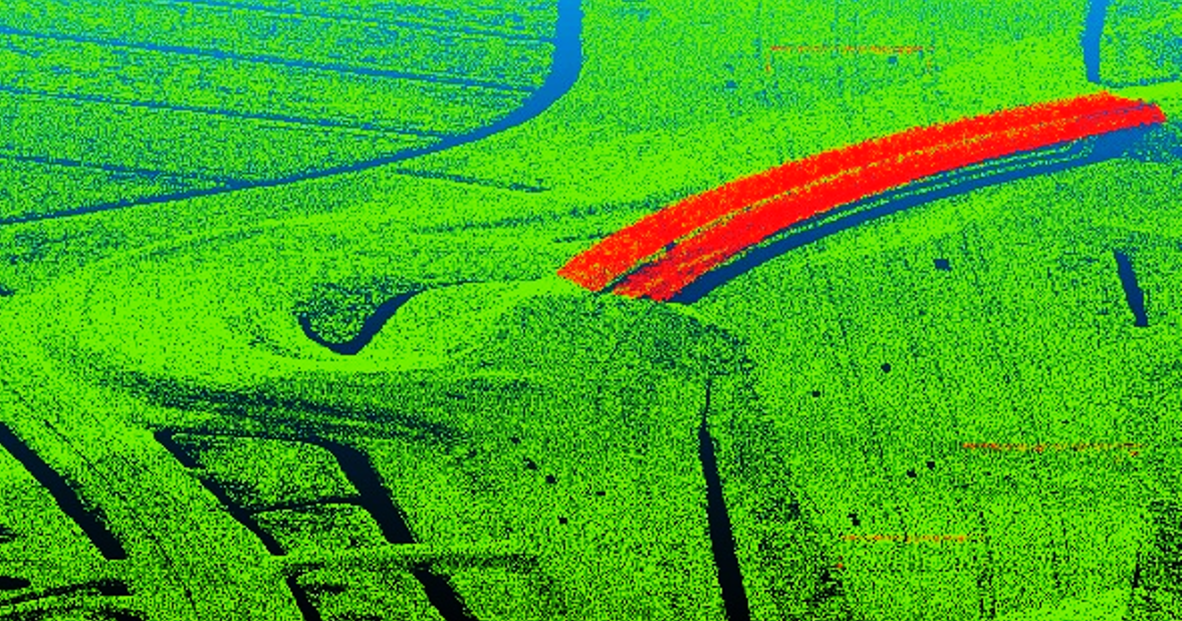
\includegraphics[width=6cm, height=3.5cm]{final_report/figs/ahn_sample_38GZ1_a.png}} \\
Knoppunt Deil, 39CZ1 & Less complex, but analogous interchange to the Knoppunt Ridderkerk. & \raisebox{-0.5\totalheight}{\textit{Please refer to Figures \ref{fig:ahnbridges}, \ref{fig:ahnsigns}, \ref{fig:ahnnwb} and \ref{fig:dtbahn}.}} \\
\toprule
\caption{Inventory of testing datasets \label{tab:inventory}}
\end{longtable}

\section{Results of processing steps}
\label{sec:results}

\textit{[Section intro to be written.]}

\subsection{Splitting NWB into NBRS}
\label{sub:r_nbrsgeneration}

\textit{[Subsection to be written.]}

\subsection{Lidar segmentation}
\label{sub:r_lidarsegmentation}

\textit{[Subsection to be written.]}

\subsection{Edge approximation}
\label{sub:r_edgeapproximation}

\textit{[Subsection to be written.]}

\subsection{Active contour optimisation}
\label{sub:r_activecontours}

\textit{[Subsection to be written.]}

\subsection{TIN construction}
\label{sub:r_tinconstruction}

\textit{[Subsection to be written.]}

\subsection{Interpolation in TIN and snapping}
\label{sub:r_interpolation}

\textit{[Subsection to be written.]}

\section{Accuracy assessment}
\label{sec:accuracy}

\textit{[Section intro to be written.]}

\subsection{Which steps affect accuracy?}
\label{sub:accuracysteps}

\textit{[Subsection to be written.]}

\subsection{TIN completeness and accuracy}
\label{sub:accuracytin}

\textit{[Subsection to be written.]}

\subsection{3D road network accuracy}
\label{sub:accuracynwb}

\textit{[Subsection to be written.]}

\section{Comparison with commercial implementation}
\label{sec:comparison}

\textit{[Section intro to be written.]}

\subsection{Overall comparison}
\label{sub:comparisonoverall}

\textit{[Subsection to be written.]}

\subsection{R-roads}
\label{sub:comparisonrroads}

\textit{[Subsection to be written.]}

\subsection{P-roads}
\label{sub:comparisonproads}

\textit{[Subsection to be written.]}